\section{Lecture 2}

\subsection{Style Guide}
We provide an informal style guide for writing mathematical proofs. 

\begin{center}
    \begin{tabular}{l|l|c}
     Goal & Knowledge & Outermost symbol \\
    \hline 
     \pbox{20cm}{Show for all $x$, $G(x)$. \\ Consider arbitrary $\hat{x}$.\\ Show $G(\hat{x})$} & \pbox{20cm}{We know for all $x$, $K(x)$ \\ In particular we know $K(\hat{t})$ for constant $\hat{t}$} & $\forall$ \\ 
    \hline 
     \pbox{20cm}{Show: exists $x$ s.t. $G(x)$. \\ We show $G(\hat{t})$} & \pbox{20cm}{We know exists $x$ s.t. $K(x)$ \\ Let $\hat{x}$ be s.t. $K(x)$} & $\exists$ \\ 
     \hline 
     \pbox{20cm}{Show $G_1$ iff $G_2$ \\ 1. Show if $G_1$ then $G_2$\\ 2. Show if $G_2$ then $G_1$} & \pbox{20cm}{We know $K_1$ iff $K_2$\\ In particular we know if $K_1$ then $K_2$\\ and if $K_2$ then $K_1$} & $\iff$ \\ 
     \hline 
     \pbox{20cm}{Show if $G_1$ then $G_2$ \\ Assume $G_1$\\ Show $G_2$} & \pbox{20cm}{We know if $K_1$ then $K_2$\\ 1. To show $K_2$ it suffices to show $K_2$\\ 2. Know $K_1$, Also know $K_2$} & $\rightarrow$ \\ 
     \hline 
     \pbox{20cm}{Show $G_1$ and $G_2$\\ 1. Show $G_1$\\ 2. Show $G_2$} & \pbox{20cm}{Know $K_1$ and $K_2$\\ 1. Also Know $K_1$ \\ 2. Also Know $K_2$} & $\wedge$ \\ 
     \hline 
     \pbox{20cm}{Show $G_1$ or $G_2$\\ 1. Assume $\neg G_1$, show $G_2$\\ 2. Assume $\neg G_2$, show $G_1$} & \pbox{20cm}{We know $K_1$ or $K_2$. Show $G$.\\
     1. Assume $K_1$, Show $G$\\ 2. Assume $K_2$, Show $G$ \\ Case split $\uparrow$} & $\vee$ \\ 
     \hline 
     \multicolumn{2}{c|}{\pbox{20cm}{Move Negation Inside, as far as possible}} &  $\neg$ \\ 
     \hline 
\end{tabular}
\end{center}

\subsection{Lattices and Fixpoints}
We define relations and their properties. 

\begin{definition}[Relation]
A binary \emph{relation} $R$ on a set $A$ is a subset $R \subset A\times A$.
The relations $R$ is:
\begin{itemize}
    \item \emph{reflexive} if for all $x$ in $A$, we have $R(x,x)$.
    \item \emph{anti-symmetric} if for all $x$ and $y$ in $A$, if $R(x,y)$ and $R(y,x)$ then $x=y$.
    \item \emph{transitive} if for all $x,y$ and $z$ in $A$, if $R(x,y)$ and $R(y,z)$ then $R(x,z)$.
    \item \emph{partial order} if $R$ is reflexive, anti-symmetric and transitive.
\end{itemize}
\end{definition}

\begin{definition}[Poset]
     A \emph{Poset} $(A,\sqsubseteq)$ is a set $A$ and a partial order $\sqsubseteq$ on $A$.
\end{definition}


\begin{example}
    Let $\NN$ be the natural numbers. The pair $(\NN,\leq)$ is a poset.
\begin{center}
     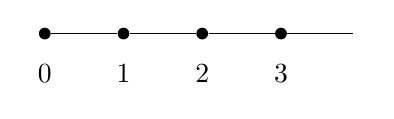
\begin{tikzpicture}[scale=1, every node/.style={circle, fill, inner sep=1.5pt}, 
    label distance=2mm]

    % Nodes
    \node[label=below:{$0$}] (0) at (0, 0) {};
    \node[label=below:{$1$}] (1) at (1 ,0) {};
    \node[label=below:{$2$}] (2) at (2, 0) {};
    \node[label=below:{$3$}] (3) at (3, 0) {};
   \node[draw=none, fill=none] (4) at (4,0) {$\hdots$};  % Dots to indicate continuation
   
    % Lines
    \draw (0) -- (1);
    \draw (1) -- (2);
    \draw (2) -- (3);
    \draw (3) -- (4);

\end{tikzpicture}
 \end{center}
\end{example}

% \begin{example}
   
   
%     \begin{figure}[h]
%         \centering
%         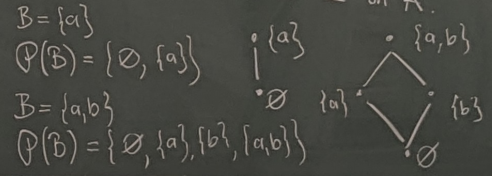
\includegraphics[width=0.7\linewidth]{images/poset.png}
%     \end{figure}
% \end{example}


\begin{example}
 For every set $B$ let $\power(B)$ be the powerset. 
 The pair $(\power(B),\subseteq)$ is a poset. E.g., for $B\coloneqq \{a\}$ (left) and for $B \coloneqq \{a,b\}$ (right).
 \begin{center}
 
     \begin{tikzpicture}[scale=1, every node/.style={circle, fill, inner sep=1.5pt}, 
    label distance=2mm]

     \node[label=right:{$\emptyset$}] (0) at (-6,0 ) {};
    \node[label=right:{$\{a\}$}] (1) at (-6,2 ) {};
    % Nodes
    \node[label=right:{$\emptyset$}] (emptyset) at (0, 0) {};
    \node[label=left:{$\{a\}$}] (a) at (-1, 1) {};
    \node[label=right:{$\{b\}$}] (b) at (1, 1) {};
    \node[label=right:{$\{a,b\}$}] (ab) at (0, 2) {};
    
    % Lines
    \draw (0) -- (1);
    
    \draw (emptyset) -- (a);
    \draw (emptyset) -- (b);
    \draw (a) -- (ab);
    \draw (b) -- (ab);

\end{tikzpicture}
 \end{center}

\end{example}


\begin{definition}[Fixpoint]
Let $(A,\sqsubseteq)$ be a poset. Let $f\colon A\to A$ be a function from $A$ to $A$.
(i) $f$ is \emph{monotone} (order-preserving, homomorphism) if for all $x$ and $y$ in $A$, if $x \sqsubseteq y$, then $f(x) \sqsubseteq f(y)$. (ii) $f$ has a fixpoint $x$ in $A$ if there exists $x$ in $A$ such that $f(x)=x$. 
\end{definition}


\begin{definition}[Upper Bound]
    Let $(A,\sqsubseteq)$ be a poset. Then (i) $x$ in $A$ is an \emph{upper bound} on a subset $B$ of $A$ if for all $y$ in $B$, it holds that $y \sqsubseteq x$; 
    (ii) $x$ is the least upper bound of $B$ if $x$ is an upper bound of $B$ and for all upper bounds $y$ of $B$, we have $x \sqsubseteq y$. We denote such $x$ by $\bigsqcup B$.
\end{definition}

\begin{definition}[Lower Bound]
    Let $(A,\sqsubseteq)$ be a poset. Then (i) $x$ in $A$ is an \emph{lower bound} on a subset $B$ of $A$ if for all $y$ in $B$, it holds that $y \sqsubseteq x$; $x$ is the greatest lower bound of $B$ if $x$ is a lower bound of $B$ and for all lower bounds $y$ of $B$, we have $y \sqsubseteq x$. We denote such $x$ by $\bigsqcap B$.
\end{definition}

\begin{example} 
    Consider the poset $(\NN,\leq)$. Then for any $B \subseteq \NN$, if $B$ is finite, $\bigsqcup B$ is well-defined and equal to $\max B$. If $B$ is infinite, then $\bigsqcup B$ does not exist. 
\end{example}

\begin{example} 
   Consider the poset $(\NN \cup \{\infty\},\leq)$ where for all $x$ in $\NN$, it holds that $x \leq \infty$. Then for all $B \subseteq \NN$, the least upper bound $\bigsqcup B$ is well-define. 
\end{example}

\begin{example} 
    Let $A$ be any set and consider the poset $(\power(A),\subseteq)$. For any subset $B$ of $\power(A)$, it holds that $\bigsqcup B = \bigcup B$ and $\bigsqcap B = \bigcap B$. 
\end{example}


\begin{definition}[Complete Lattice]
    Poset $(A,\sqsubseteq)$ is a \emph{complete-lattice} if for all $B \subseteq A$, both $\bigsqcap B$ and $\bigsqcup B$ exist.
\end{definition}
\begin{example}
    Let $(A,\sqsubseteq)$ be a complete-lattice. Then: $\bigsqcup A = \top$, $\bigsqcap A = \bot$, $\bigsqcup \varnothing = \bot$, and $\bigsqcap \varnothing = \top$
\end{example}

% \begin{definition}
%     Let $(A,\sqsubseteq)$ be a poset and let $F$ be a function from $A$ to $A$. 
%     Then $x$ in $A$ is a pre-fixpoint of $F$ if $x \sqsubseteq F(x)$ and is a post-fixpoint of $F$, if $F(x) \sqsubseteq x$. 
% \end{definition}




\begin{theorem}[Knaster-Tarski]
\label{thrm:knaster}
    For every complete lattice $(A,\sqsubseteq)$ and monotone function $f$ on $A$, it holds that: (i) $\bigsqcup \{x\in A| x \sqsubseteq f(x)\}$ is the unique greatest fixpoint of $F$; (ii) $\bigsqcap \{x \in A| f(x) \sqsubseteq x\}$ is the unique least fixpoint of $f$. 
\end{theorem}


\begin{exercise}
        Prove the Knaster Tarski Theorem (Theorem \ref{thrm:knaster}).
\end{exercise}


